\documentclass[12pt]{article}
\usepackage[a4paper, total={16cm,25cm}]{geometry}
\usepackage{titlesec}
\usepackage{graphicx}
\usepackage{float}
\PassOptionsToPackage{hyphens}{url}\usepackage{hyperref}
\usepackage{fancyhdr}
\setlength{\headheight}{30pt}
\pagestyle{fancy}
\fancyhead[L]{HSI使用說明書}
\fancyhead[R]{\leftmark}
\renewcommand{\headrulewidth}{2pt}
\usepackage{amsmath}
\usepackage{latexsym}
\usepackage{multirow}
\graphicspath{ {./images/} }
\usepackage[backend=biber, citestyle=numeric, bibstyle=numeric, sorting=none]{biblatex}
\addbibresource{ref.bib}
\usepackage{mathspec}   %加這個就可以設定字體
\usepackage{xeCJK}       %讓中英文字體分開設置
\setCJKmainfont{Noto Serif CJK TC} %設定中文為系統上的字型
\newCJKfontfamily[chineseSans]\CJKsans{Noto Sans CJK TC}
\setmainfont{Roboto Serif}
\setsansfont{Roboto}
\setmonofont{Roboto Mono}
\XeTeXlinebreaklocale "zh"             %這兩行一定要加,中文才能自動換行
\XeTeXlinebreakskip = 0pt plus 1pt     %這兩行一定要加,中文才能自動換行
\renewcommand{\baselinestretch}{1.35}
\renewcommand{\figurename}{圖}
\renewcommand{\tablename}{表}
\renewcommand{\abstractname}{摘要}
\renewcommand{\contentsname}{目錄}
\renewcommand{\listtablename}{表格目錄}
%\renewcommand*{\bibfont}{\footnotesize}
\titleformat*{\section}{\Large \bfseries}
\titleformat*{\subsection}{\large \bfseries}
\titleformat*{\subsubsection}{\bfseries}

\begin{document}
    \thispagestyle{empty}\null\vspace{5cm}\noindent{\Large HyperSpectral Imaging System}\newline
    {\large 軟體操作使用說明書}\newpage
    \tableofcontents\newpage
    \section{啟動軟體}
    本軟體尚未編譯為可執行檔,請開啟並執行HIS.lvproj中的main.vi,即可啟動軟體。軟體啟動時,會自動偵測是否能成功連接iXon相機,若連接失敗,系統判定並未連接iXon,則軟體會出現訊息視窗,
    並自動進入讀取模式。
    
    一旦軟體啟動,並成功連接iXon,系統即會自動開啟iXon的TE Cooler,此時使用者即可自行輸入欲達到的溫度,待系統完成降溫且溫度穩定後,Cooler燈號才會轉為綠色。
    當系統硬體都成功連接後,軟體會自動進入影像與掃描設定的模式。此時在畫面左半側的系統控制區,多數的控制元件都會啟動,少數呈現刷白的控制元件是無法使用的。此時在影像與掃描設定模式下,
    可以對系統的影像、掃描參數進行設定,為掃描進行準備。

    同時,在畫面的右半側,共計有四個顯示螢幕,是軟體的影像資料檢索介面。該介面此時也是處於啟動狀態,能夠幫助使用者檢視當前設定下的影像資料。
    \begin{figure}[h]
        \centering
        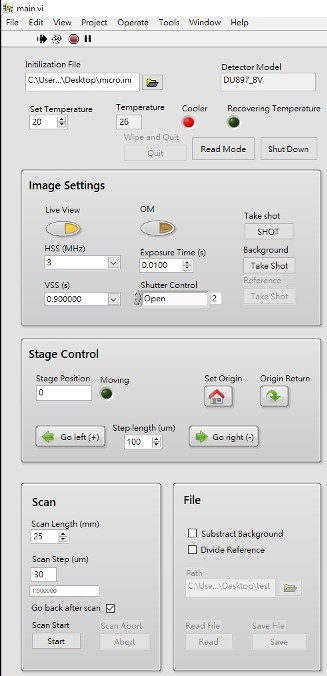
\includegraphics[width=0.33\linewidth]{settingPanel.jpeg}
        \caption{系統控制區。}
    \end{figure}
    \begin{figure}[h]
        \centering
        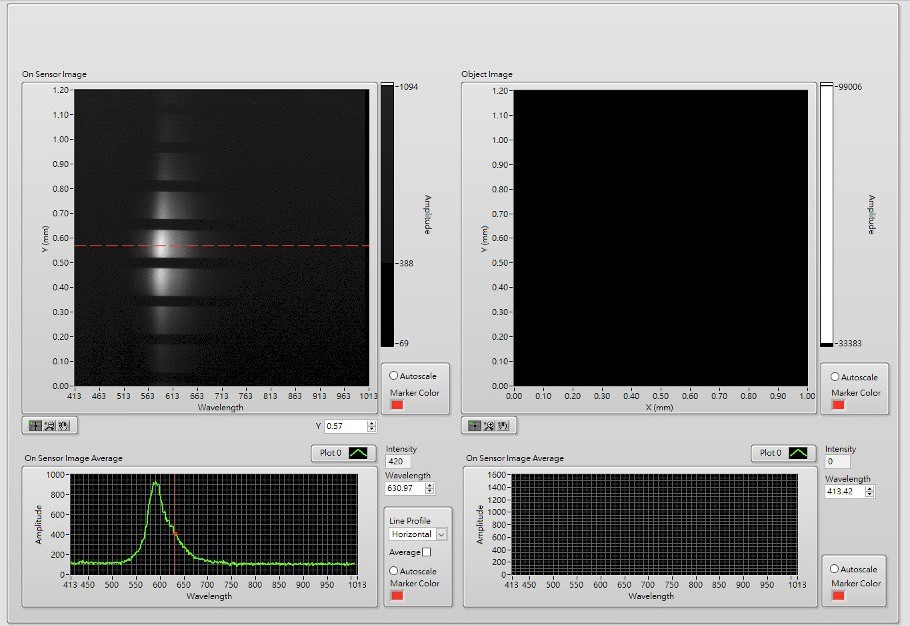
\includegraphics[width=0.75\linewidth]{browsePanel.jpeg}
        \caption{影像資料檢索介面。}
    \end{figure}

    \section{系統控制區}
    \subsection{啟動與模式控制區}
    在本區中選取系統起始參數檔(init file),一般來說使用者不需特別理會起始參數檔。若要切換起始參數檔,必須將軟體關閉後,重新指定參數檔路徑,再開啟軟體。

    若系統啟動後成功連接iXon,本區也會顯示出iXon的型號。同時,使用者可以在set temperature處設定欲使sensor達到的降溫目標,一旁的temperature則會顯示出目前的溫度。等到降溫完成且溫度穩定後,cooler status燈號才會轉為綠色。
    \footnote{請參閱iXon說明書了解合適的降溫目標溫度。}

    本區最重要的為下排的三個按鍵: quit, read mode, shut down。剛啟動時quit會被關閉,無法按下。在使用者完成掃描後,該按鍵可以讓使用者退出瀏覽模式並回到影像與掃描設定模式。
    任何時候若按下read mode,系統會直接進入讀取模式,方便使用者在只需要讀取檔案時使用。任何時候按下shut down,則會將系統關閉。請注意,關閉系統時軟體會先關閉iXon cooler,直到溫度
    回到0度c以上後,才會完全關閉系統。
    \subsection{Image Settings影像設定區}
    使用者可以在此區已各個選單調整以下影像參數:
    \begin{itemize}
        \item HSS: (Horizontal shift speed)代表的是iXon sensor橫向的讀取速度,單位為MHz,較慢的設定會等比例的加長掃描時間,一般來說將設定維持在3MHz即可。\footnote{請參閱iXon說明書了解何時須使用其他值。}
        \item VSS: (Vertical shift speed)代表的是iXon sensor直向的讀取速度,在某些情形下該參數設定較慢(如0.9s)會讓影像品質變好,不過liveview時將此設定為較快的值會有效增進frame rate。
        \item Gain: 從此下單選單選取增益。可用的增益選項是由iXon相機所決定的。增益的模式則是由init檔所決定。
        \item Exposure Time: iXon的曝光時間。
        \item Shutter Control: 開啟或關閉iXon內建的快門。請參閱iXon說明書了解其他快門模式。請先將快門開啟再開始掃描,勿使用自動快門模式。
    \end{itemize}
    另外,使用者可以在此區進行以下單張影像的擷取:
    \begin{itemize}
        \item Take Shot: 以當前的影像參數擷取一張照片,並顯示於影像資料檢索區的右側大螢幕。
        \item Background: 按下後,系統會關閉快門,以當前的影像參數擷取一張照片,並顯示於影像資料檢索區的右側大螢幕。該張影像將儲存於記憶體中,掃描結束後會用於三維影像資料的背景雜訊移除,請參閱節\ref{sec: bkg/ref}。
        \item Reference: 按下後,系統會開啟快門,以當前的影像參數擷取一張照片,並顯示於影像資料檢索區的右側大螢幕。該張影像將儲存於記憶體中,掃描結束後會用於三維影像資料的反射率計算,請參閱節\ref{sec: bkg/ref}。
    \end{itemize}

    該區有兩個重要按鍵,首先是liveview,按下後會亮起橘黃色燈號,表示目前正在實時顯示iXon sensor上的畫面,該畫面會呈現在影像資料檢索介面的左側大螢幕上。liveview時所採用的影像參數,就是當前該區所設定的參數。
    再按一次liveview鍵,liveview就會停止同時案件的燈號也會熄滅。若是因為啟動liveview,或是擷取其他單張影像,因而有影像資料顯示在兩處大螢幕上時,就可以使用節\ref{sec: browse tool}中的影像資料檢索工具。
    \subsubsection{OM影像}
    另一個按鍵是OM,按下後同樣會亮起燈號,並在影像資料檢索介面的右側開啟一個OM顯示幕,以方便使用者觀測樣品的實際樣貌。OM畫面上的兩條白色橫虛線,標示出線光譜儀入射狹縫的視野上下界,
    而中間的垂直白色虛線,則是標示出目前入射狹縫所觀測的位置。
    
    此時OM已在進行liveview,該介面上另有OM liveview影像參數的設定選單,分別是感光度ISO與曝光時間Exposure Time,同時亦會有ROI掃描的相關控制介面出現,請參閱節\ref{sec: roi scan}。
    \begin{figure}[h]
        \centering
        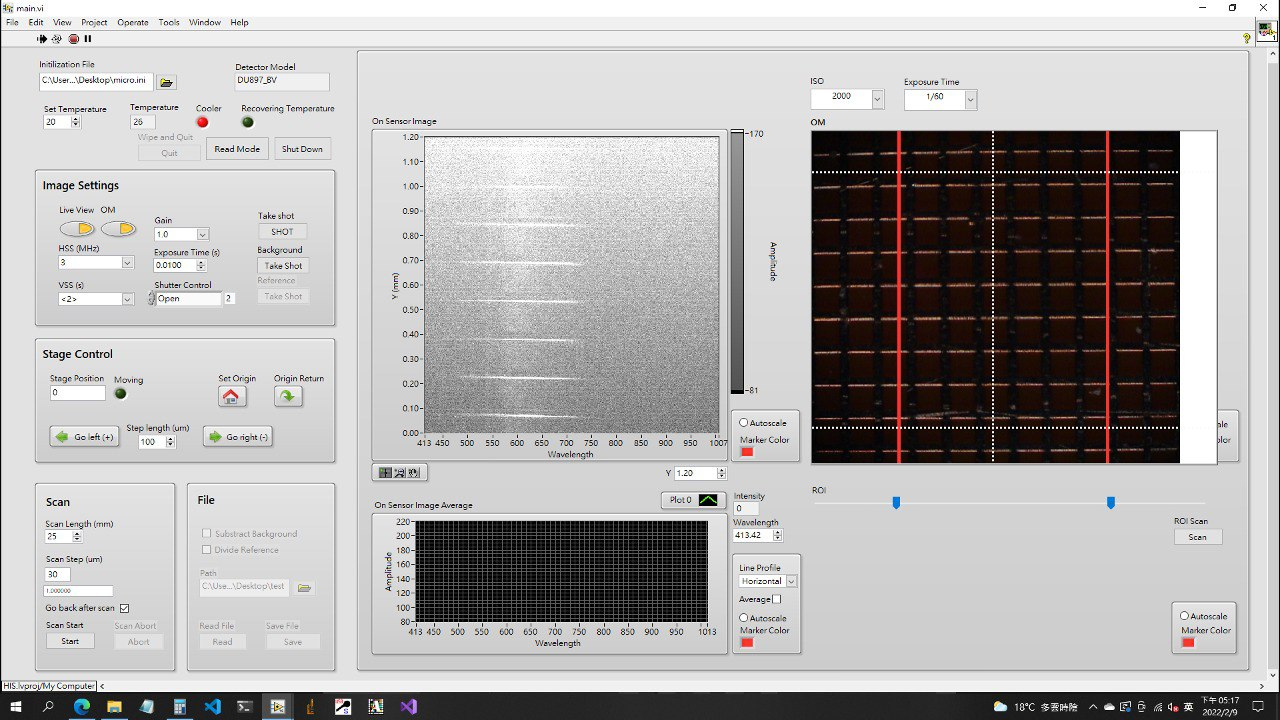
\includegraphics[width=\linewidth]{roi.jpeg}
        \caption{OM與iXon同時liveview畫面。}
        \label{fig: liveview}
    \end{figure}

    \subsection{Stage Control載台控制區}
    本區會顯示電動載台目前的位置與狀態。同時使用者可以在這裡移動電動載台,Step length設定欲移動的距離,接著按下向左/向右鍵,電動載台即會向該方向移動設定的距離。該處所顯示的距離皆是電動載台的座標值,是pulse數,
    與真實距離的關係視division number而定。同時在向左/向右鍵的一旁,會顯示載台在該方向的software limit,載台不會移動到超過software limit的位置。

    本區另有Set Origin與Go Home兩個按鍵。Set Origin的功能是將電動載台目前的所在位置設定為座標0。而Go Home則是在使用者認為電動載台座標偏移時,用來重新校正用。
    若按下此鍵,電動載台會自動回到其機械原點,接著回到使用者上次所定義的座標0處。若使用者僅是在操作過程中單純要回到座標原點,建議調整Step length為目前位置並往原點移動即可。
    \subsection{Scan掃描設定區}
    在本區設定掃描的距離,以及掃描步進(每次影像擷取之間要移動的距離)後,即可按下Scan鍵開始掃描。請注意,掃描的方式是從載台當前的位置開始,向載台座標的負方向(右側、ccw方向)進行指定距離的掃描。
    Scan step下方的小欄位,會顯示依據目前的division number可設定的最小步進。請注意,與載台控制區不同的是,此處的長度設定都是實際距離,而非電動載台的pulse座標。
    \subsection{ROI掃描}\label{sec: roi scan}
    當影像設定區的OM開啟時(如圖\ref{fig: liveview}所示),OM螢幕下方會有一個橫條,上方有兩個拉趕,使用者拉動拉趕時,OM螢幕上的紅色垂直線會跟著拉趕左右移動。
    使用者可以用這兩條紅線框取OM影像上欲掃描的區域,接著按下ROI Scan,系統就會自動完成該區域的掃描,掃描完成後,載台會再移動至使用者進行框取時載台的位置,而非掃描起始的位置。

    請注意,以ROI Scan按鍵開始掃描時,掃描步進仍然是以掃描設定區Scan step的設定為準。
    \subsection{Data資料檢索區}
    本區只有在掃描結束,進入瀏覽與存檔模式時,才能夠使用。檢視影像資料時,可以在此選擇是否要將影像資料減去背景雜訊並/或除以參考光譜。若掃描前有拍攝背景光譜與/或參考光譜,相應的選項才會出現。
    同時,也可以在此選擇讀檔或存檔的路徑。
    \section{掃描}
    按下掃描設定區或ROI掃描的Scan鍵後的,系統就會開始進行掃描。請注意,請先將快門開啟再開始掃描,勿使用自動快門模式。掃描結束後是否會回到起始位置,則可由使用者在掃描設定區設定。
    請注意,掃描時,軟體介面上的所有選項皆會被關閉無法操作,包括影像資料檢索工具,也都無法使用,必須按下Scan Abort才能停止掃描,並進入瀏覽模式中。
    
    掃描過程中,檢索介面的左側螢幕會實時顯示iXon的影像資料擷取,右側螢幕則會顯示樣品已被掃描的部分之樣貌,也可作為掃描進度的判斷。同時,畫面上方會顯示出目前已拍攝的影像張數/總共需拍攝的影像張數。
    請注意,右側螢幕所顯示的樣品影像,因為需填滿正方形的螢幕,因此顯示比例會明顯與實物不同。
    \begin{figure}[h]
        \centering
        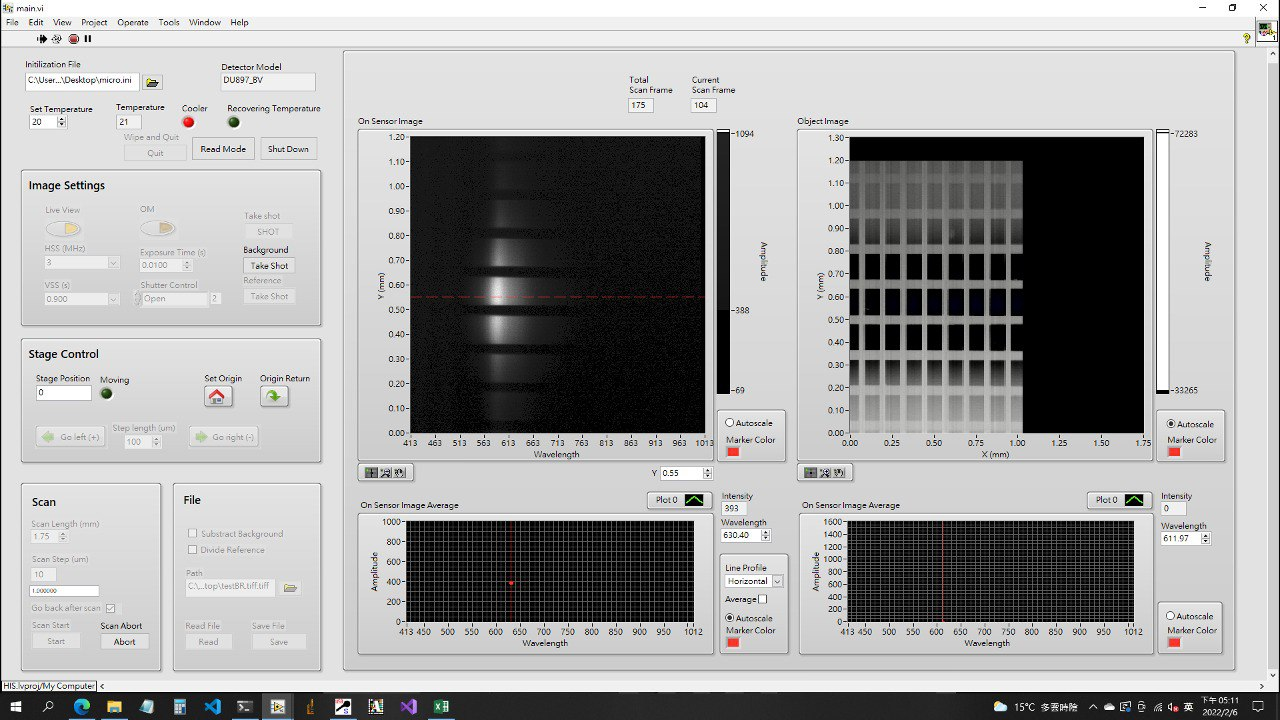
\includegraphics[width=\linewidth]{scanning.jpeg}
        \caption{掃描時。}
        \label{fig: scanning}
    \end{figure}
    \section{瀏覽與存檔}\label{sec: browse}
    掃描結束後,系統會進入瀏覽模式,在此可以使用所有的影像資料檢索工具。在右側的螢幕上,會顯示出掃描過後樣品在指定波長下的影像,右側螢幕的上方有一個拉趕,滑動此拉趕可以調整指定波長,
    若一旁的bandwidth設定為非0的值,則右側螢幕會顯示出指定波長加/減該值的波長範圍內的平均影像。

    右側螢幕下方有一個Fill screen/Real ratio切換鍵,按下後可以讓右側螢幕顯示比例自動調整,使樣品影像的比例看起來與實物較相似。

    在本模式下,以滑鼠點選右側螢幕上的位置,螢幕上就會顯示出滑鼠點擊的位置,與該位置上的垂直線,下方的小螢幕就會顯示出該位置的光譜,而該垂直線所在位置的線掃描光譜,則會顯示在左側的大螢幕上。
    X、Y兩個小欄位,也會顯示出目前滑鼠點選的位置。
    此時左側的小螢幕,就是影像資料資料檢索工具,可以幫助使用者檢視左側螢幕上影像資料的line profile。

    使用者若要將目前顯示中的掃描資料儲存,請先在Data資料檢索區選擇欲儲存的路徑\footnote{請在選擇路徑的彈出視窗中,找到欲儲存的位置後,輸入檔名,不必加入副檔名。},再按下save鍵即可。
    此時按下quit鍵,就會回到影像與掃描設定模式。
    \subsection{影像檢索工具}\label{sec: browse tool}
    \subsubsection{影像檢索}
    以滑鼠在左側螢幕上點選,點選位置上會出現一條直線,該直線的line profile會被呈現在下方的小螢幕上。小螢幕旁的Line profile選單,可以調整該直線的方向是垂直或水平。大螢幕下方的小欄位,
    會顯示出該滑鼠點選的位置。
    \subsubsection{光譜檢索}
    無論在左或右的兩個小螢幕,當有光譜或Line profile顯示於其上時,只要用滑鼠在上點擊,軟體就會在點擊位置上畫出一條垂直線,該垂直線所在的x軸座標,會顯示在一旁的小欄位上。
    同時,軟體會在該x軸座標上的資料點,畫上一圓點,並顯示出該資料點的直在小螢幕旁的小欄位。
    \par \noindent 每個螢幕旁都會有marker color與autoscale兩個控制項。按下marker color可以選擇該螢幕上的位置標示所要顯示的顏色,按下autoscale則可以開啟/關閉顯示強度的autoscale。
    影像資料檢索介面中,每一個附有上下兩個小按鈕數字顯示欄,都可以用上下小按鈕或鍵盤輸入來調整其值,螢幕上的位置標示也會跟著輸入值改動。
    \begin{figure}[h]
        \centering
        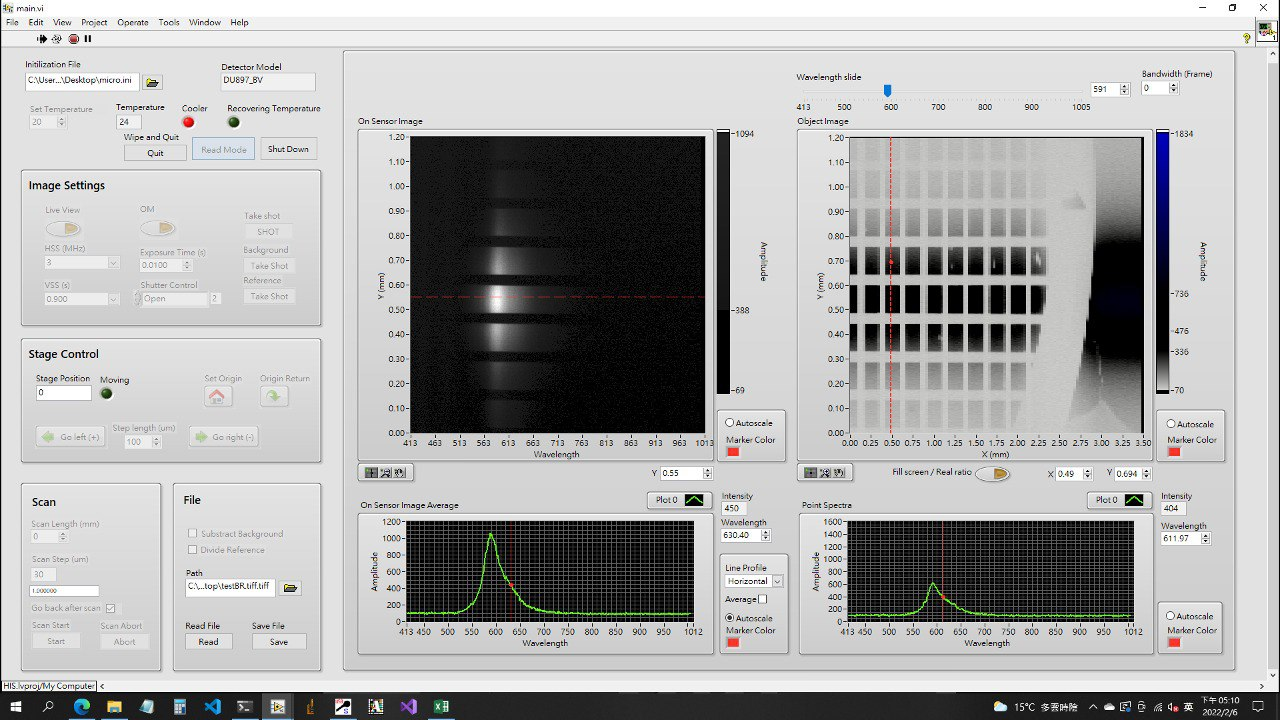
\includegraphics[width=\linewidth]{readmode.jpeg}
        \caption{影像資料瀏覽。}
        \label{fig: browsing}
    \end{figure}
    \subsection{背景與參考光譜}\label{sec: bkg/ref}
    只有在影像資料中存有背景/參考光譜時(無論是從檔案讀入的資料或是掃描後的資料),資料檢索區的「背景光譜減除」與「除以參考光譜」選項才會能被使用。同時,若勾取「除以參考光譜」,
    則「背景光譜減除」也會自動被一並勾取。
    \begin{figure}[h]
        \centering
        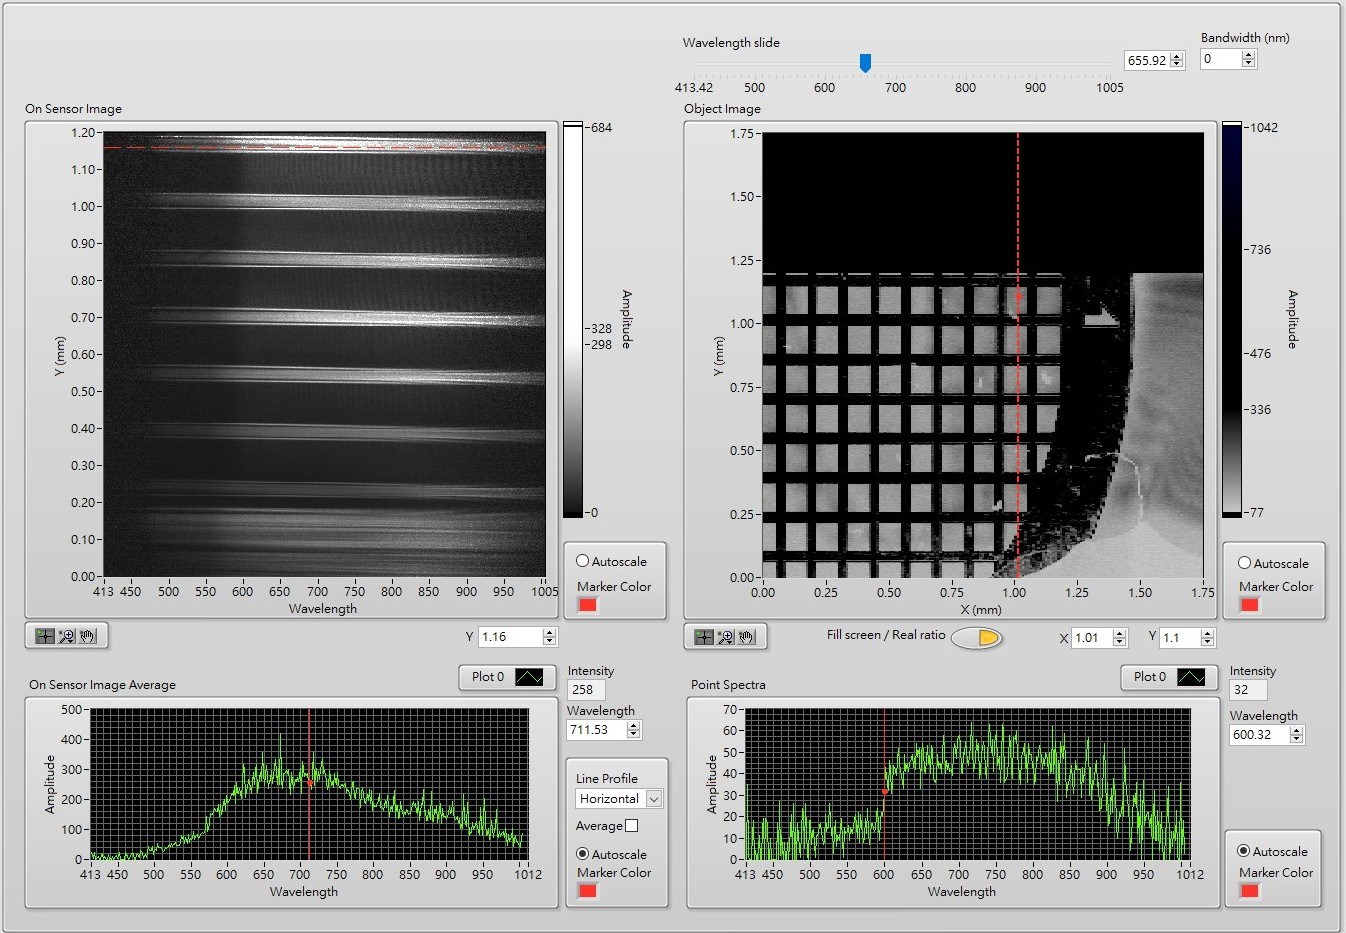
\includegraphics[width=0.75\linewidth]{reflection (2).jpeg}
        \caption{檢視反射率。}
        \label{fig: reflection}
    \end{figure}
    \section{讀檔}
    在掃描結束,或是按下read mode,軟體進入瀏覽模式後,只要在Data資料檢索區的Path選擇欲讀取的檔案,再按下Read file,軟體就會將影像資料讀入,有如剛結束掃描一般,所有操作皆會與節\ref{sec: browse}相同。
    同時,從影像資料中讀出的各個影像參數,則會顯示於影像設定區的各個欄位中。

    同樣地,此時按下quit鍵,就會回到影像與掃描設定模式。
\end{document}